\chapter{Constructions}\label{chap:constructions}

\begin{epigraph}{14em}{Hermann Weyl}
	The introduction of numbers as \\
	coordinates is an act of violence.
\end{epigraph}

The focus on this chapter will be on three important constructions of exotic spheres -- as total spaces of sphere bundles, as the boundary of a ``plumbing'' of disk bundles along a tree, and as the ``link'' of an isolated singularity of a holomorphic functions. In later sections, it will be possible to directly compute invariants of these constructed manifolds to understand which elements of $\Theta^n$ these manifolds correspond to. As with many challenging topics in math, an abundance of examples helps alleviate some of the complexity, and we hope this chapter can do this for exotic spheres.
That being said, a time-pressed reader need only read \cref{sec:plumbing}, since this is a simple direct construction which will suffice for a classification of exotic spheres in \cref{chap:classification}.

The basic ingredients for a good exotic sphere construction includes the following:
\begin{enumerate}[(a)]
	\item A general class of non-trivial smooth manifolds which have highly-connected boundary.
	\item A simple criterion for when this boundary is homotopy equivalent to a sphere.
	\item Some geometric structure on the bounding manifold which simplifies the computation of some topological invariants.
\end{enumerate}


bounding manifold of a homotopy sphere can't be contractible

\pagebreak
\section{Milnor Spheres}\label{sec:milnor-spheres}

We will begin with the classical construction of exotic spheres as total spaces of sphere bundles over a sphere, starting with Milnor's original construction of an exotic 7-sphere in \cite{milnor1956manifolds}. To see how spheres can arise as total spaces of sphere bundles over a sphere, we will review the Hopf bundles -- these construct ordinary spheres. By ``twisting'' Hopf bundles in sufficiently high dimension, we will be able to get exotic spheres.

The simplest Hopf bundle is the real Hopf bundle, which constructs the circle $S^1$ as the total space of an $S^0$ bundle over $S^1$. Topologically, this is just the double cover of $S^!$, but it is instructive to consider this simple case in the same manner as the complex and quaternionic Hopf bundles which be considered next.
Consider the projection map
\[
	\lkxfunc{\pi_\R^n}{S^n}{\RP^n}{(x_1,\ldots, x_{n+1})}{[x_1:\cdots: x_{n+1}]}
\]
which sends a point on a sphere $S^n\subset \R^{n+1}$ to the line passing through the point and the origin. This is a double cover since antipodal points are sent to the same line -- in fact it is the universal covering space of $\RP^n$. The fibers of this map are then $S^0$.
When $n=1$, there is an isomorphism $\RP^1\approx S^1$ by stereographic projection, and so $\pi_\R^1$ is the $S^0$-bundle
\[
	S^0 \lkxto S^1\lkxto S^1.
\]
This is the \defn{real Hopf bundle}[Hopf bundle (real)]. Note that real Hopf bundle $\pi_\R^1$ can be interpreted as the boundary of the compact M\"obius bundle $M$, which is a $D^1$-bundle over $S^1$.
We can directly construct $M$ from $\pi_\R^1$ by taking the $M = S^1\times_{\Z/2} D^1$ to be the bundle associated to the action of $\Z/2$ by reflection on $D^1\subset \R$. There is also an embedding of $M$ into a surface we are familiar with -- in fact $M$ is homeomorphic to the complement of an open disk $\Int(D^2)$ in the real projective plane $\RP^2$.

Advancing from $\R$ to $\C$, we consider the projection map
\[
	\lkxfunc{\pi_\C^n}{S^{2n+1}}{\CP^n}{(z_1,\ldots, z_{n+1})}{[z_1:\cdots: z_n]}
\]
where we interpret $S^{2n+1}\subset \R^{2n+2}$ as a subset of $\C^{n+1}$.
In this case, the fibers consist of unit norm complex numbers, i.e. the set of phase changes $S^1=\{e^{i\theta} : \theta\in \R\}$ which is diffeomorphic to $S^1$.
When $n=1$, there is an isomorphism of the Riemann sphere $\CP^1\cong S^2$ by stereographic projection. This gives the us the infamous \defn{complex Hopf bundle} $\pi_\C^1$
\[
	S^1 \lkxto S^3 \lkxto S^2.
\]
By letting $S^1\cong \U_1$ act as rotations on the complex unit disk $D^2\subset \C$, we get an associated $D^2$-bundle $E = S^3\times_{\U_1} D^2$.

Similarly to the real case, the total space of this associated bundle turns out to be a complex projective plane $\CP^2$ with an open disk $\Int(D^4)$ removed. Recall that $\CP^n$ can be formed inductively by glueing a $2n$-cell $D^{2n}$ to $\CP^{n-1}$ by the map $\pi_\C^{n-1} : \partial D^{2n} \to \CP^{n-1}$, this gives the usual cell structure on $\CP^n$ with a single cell in each even dimension.
We can arrange the open disk $\Int(D^4)$ being removed from $\CP^4 = S^2\cup_{\pi_\C^1} D^4$ to lie strictly in $D^4$. Removing this disk then gives a $D^2$-bundle over the boundary $S^2$.

\begin{remark}
	Unlike the real and complex numbers, the quaternions $\HH$ are not a field since they are not commutative. In this thesis, we define quaternionic projective space $\HP^{n}$ as the quotient of $\HH^{n+1}$ by \emph{right} multiplication by $\HH$.
\end{remark}

Now in the final case of the quaternionic plane $\HH$, we have a projection map
\[
	\lkxfunc{\pi_\HH^n}{S^{4n+3}}{\HP^n}
\]
where we consider $S^{4n+3}\subset \HH^{n+1}$. This bundle with fibers given by the set of unit quaternions $S^3\subset \HH$.
In the case $n=1$, the difeomorphism $\HP^1\cong S^3$ gives the \defn{quaternionic Hopf bundle}[Hopf bundle (quaternionic)]
\[
	S^3 \lkxto S^7 \lkxto S^4.
\]
Since the fiber $S^3$ has a Lie group structure $\SU_2$, we can do the same associated bundle construction to get a $D^4$-bundle which bounds the total space of the quaternionic Hopf bundle $\pi_\HH^1$. The total space of this bundle is diffeomorphic to the complement of an open disk $\Int(D^8)$ in quaternionic projective plane $\HP^2$ by a similar argument to what was done in the complex case.

In the coming section, we will try to generalize the Hopf bundles, twisting the bundle just enough so that the total space has a non-standard smooth structure but not so much that it ceases to be homeomorphic to a sphere.
Of course, this will lose some of the elegant and canonical geometric structure of the Hopf bundles, but it is still useful to keep the Hopf bundles in mind throughout.

\subsection{Sphere Bundles and the Euler Class}

Let us suppose we had a general oriented sphere bundle of the form
\begin{equation}\label{eq:general-spherical-fibration}
		S^{n-1}\lkxto M \lkxto S^n.
\end{equation}
When will $M$ be homotopy equivalent to a sphere? There are a few ways to proceed here -- for instance we could use the homology Serre spectral sequence and the Hurewicz map in order to compute the homology of $M$ from the data of the attaching map $\delta : \pi_n(S^n) \to \pi_{n-1}(S^{n-1})$. A simpler approach, more in line with the theme of this thesis, involves the Euler class constructed in \cref{sec:euler-class}.

\begin{theorem}[Gysin Sequence]
	Whenever we have a bundle $S^{n-1} \to E\to B$ over a simply-connected base $B$, there is an exact sequence known as the \defn{Gysin sequence} 
	\[
		\cdots \lkxto \H^{k-n}(B)\lkxto[e\smile] \H^k(B)\lkxto[p^*] \H^k(E)\lkxto H^{k-n+1}(B)\lkxto \cdots
	\]
	where $e\in \H^n(B)$ is the Euler class of the bundle $p : E \to B$.
\end{theorem}
\begin{proof}
	See Section 4.D of \cite{hatcher2002topology} or Theorem 17.9.2 of \cite{dieck2008algebraic}.
\end{proof}

In the case of the bundle of \cref{eq:general-spherical-fibration}, the Gysin sequence gives us exact sequences of the form
\[
	\cdots \lkxto \H^\ell(S^n) \lkxto \H^{\ell}(M) \lkxto \H^{\ell - n+1}(S^n) \lkxto[e\smile] \H^n(S^n) \lkxto \cdots
\]
When $\ell$ is not $0,n-1,n,$ or $2n-1$, the terms $\H^\ell(S^n)$ and $\H^{\ell - n+1}(S^n)$ vanish, implying that $\H^\ell(M)$ is trivial. As a connected oriented $2n-1$ manifold, we know that $\H^0(M)$ and $\H^{2n-1}(M)$ are both isomorphic to $\Z$. In the problematic case of $\ell = n-1$ or $n$, note that we have the exact sequence
\[
	 0 \lkxto \H^{n-1}(M) \lkxto \H^0(S^n) \lkxto[e\smile] \H^n(S^n) \lkxto \H^n(M) \lkxto 0
\]
Here $H^0(S^n)$ and $H^n(S^n)$ are both isomorphic to $\Z$, with the Euler class acting as a multiplication map. It follows that terms $\H^{n-1}(M)$ and $\H^n(M)$ vanish if and only if multiplication by the Euler class is an isomorphism. This forces the Euler number to be $\pm 1$.

\begin{proposition}\label{prop:homotopy-type-spherical-bundle}
	The total space of a bundle $S^{n-1} \to M \to S^n$ is a homotopy sphere if and only if the Euler number is $e=\pm 1$.
\end{proposition}

\begin{remark}
	There is a nice geometric example of the condition $e=\pm 1$ for the Hopf bundle.

	The crux of the interpretation is \cref{thm:euler-number-self-intersection}, which tells us that the self-intersection number of a submanifold $N\subset M$ is the Euler number of a tubular neighborhood.
	In the case of the complex Hopf bundle, recall that $\CP^2\setminus \Int(D^4)$ is a $D^2$-bundle over $S^3$ which bounds the complex Hopf bundle. This is exactly the bundle associated to the action of $S^1\cong \U_1$ on $D^2$. Let us call the total space $W$, and denote the Hopf bundle $p : S^3 \to S^2$ and $\overline{p} : W \to S^2$ for the $D^2$ bundle.
	\[
	\begin{tikzcd}
		D^2 & W & \\
				& & S^2\\
		S^1 & S^3 &
		\arrow["\partial"', from=1-1, to=3-1]
		\arrow["\partial"', from=1-2, to=3-2]
		\arrow["p"', from=3-2, to=2-3]
		\arrow["\overline{p}", from=1-2, to=2-3]
	\end{tikzcd}
\]
While $p$ certainly does not have a section, $\overline{p}$ does -- since the $0\in D^2$ is a fixed point of the $\U_1$ action we have a zero section. The removal of the open $4$-disk from $\CP^2$ does not affect lower dimensional homology groups of $\CP^2\setminus \Int(D^4)$. 
Furthermore, the embedding by the zero-section of $\overline{p}$ of $S^2\subset W$ generates the middle-dimensional homology $\H^2(W)$. The plane bundle associated to the Hopf bundle $p$ is then a tubular neighborhood of $S^2\subset W$ and so by \cref{thm:euler-number-self-intersection}, the Euler number of the Hopf bundle is the self-intersection of $S^2$ in $W$. However, the intersection form of $\CP^2$ is the same as the intersection form of $W$, it is $(1)$ by \cref{prop:intersection-form-complex-projective-plane}. This means that the Euler class of the Hopf bundle is $\pm 1$ which agrees with \cref{prop:homotopy-type-spherical-bundle}.
\end{remark}

\begin{remark}
	When building manifolds as total spaces of sphere bundles, it is usually easier to work with first with a vector bundle. This allows for a natural construction of both a sphere bundle and a bounding disk bundle given a Riemannian structure. Working with vector bundles, especially when the base manifold is a sphere as well is generally easier because we can classify vector bundles by the clutching construction as a homotopy group of the structure group. 

	In the case that the fiber $S^{n-1}$ is $S^0, S^1, S^3,$ there is a Lie group structure on $S^{n-1}$ which acts on $\R^{n}$ so we can always associate a rank $n$ vector bundle to an $S^{n-1}$ bundle. When the fiber does not have a Lie group structure, we can still form sphere bundles out of vector bundles, but it is not necessarily true that all sphere bundles arise in this way.
\end{remark}

\subsection{Milnor's Exotic Spheres in 7-Dimensions}

\begin{proposition}\label{prop:3rd-homotopy-SO4}
	There is an isomorphism $\pi_3(\SO_4)\cong \Z\oplus \Z$.
\end{proposition}
\begin{proof}
	\todo{finish this up}
\end{proof}

\begin{definition}
	For each $(i,j)\in \pi_3(\SO_4)$, the \defn{Milnor sphere}[Milnor sphere (7-dimensional)] $\Sigma_{i,j}^7$ is the total space of the bundle associated to the clutching function $(i,j)$. Let $p_{i,j} : \Sigma_{i,j}^7 \to S^4$ be the bundle map.
\end{definition}

\begin{proposition}\label{prop:milnor-spheres-homeomorphic-to-spheres}
	When $i+j=1$, the Milnor sphere $\Sigma_{i,j}^7$ is homeomorphic to $S^7$.
\end{proposition}

Of course, by \cref{prop:homotopy-type-spherical-bundle}, this follows by the $h$-cobordism theorem since $\Sigma_{i,j}^7$ has the homotopy type of $S^7$. However, at the time of Milnor's construction the $h$-cobordism had not been proved so he directly proved homeomorphism using Reeb's theorem \cref{thm:reeb}.

\begin{proof}[Proof of \cref{prop:milnor-spheres-homeomorphic-to-spheres}]
	Identifying $S^3\subset \HH$ with the set of unit norm quaternions, the clutching function $S^3 \to \Aut(\HH)$ corresponding to $(i,j)$ is $v\mapsto u^ivu^j$. Consider the charts
	\[
		U_0 = \{ [u_0:1] \mid u_0\in \HH\}\quad\textrm{and}\quad U_\infty = \{ [1:u_\infty] \mid u_\infty\in \HH\}
	\]
	on the sphere $S^4=\HP^1$. Note that the change of coordinate map is $u_\infty=u_0^{-1}$.Then, the Milnor sphere is homeomorphic to the quotient
	\[
	\Sigma^7_{i,j} = (U_0 \times S^3)\cup_h (U_\infty\times S^3)
	\]
	where $h$ is the map identifying $(u_0,v_0)\in U_0\times S^3$ with
	\[
		h(u_0,v_0)= \left(u_0^{-1}, \frac{u_0^iv_0u_0^j}{\|u_0\|^{i+j}}\right) = \left(u_0^{-1}, \frac{u_0^i (v_0u_0) u_0^{-i}}{\|u_0\|}\right) = (u_\infty, v_\infty),
	\]
	where the second equality follows from $i+j=1$.
	Note that $h$ acts as a change of coordinate function between the two ``hemispheres'' $U_0\times S^3$ and $U_\infty\times S^3$.
	Now, consider the real function $f : U_\infty\times S^3\to \R$ defined by
	\[
		f(u_\infty, v_\infty) = \frac{\Re(v_\infty)}{\sqrt{1+\|u_\infty\|^2}}.
	\]
	Under a change of coordinates, this function is
	\[
		f(u_\infty, v_\infty) = \frac{\Re(u_0^i(v_0u_0)u_0^{-i})/\|u_0\|}{\sqrt{1+\|u_0^{-1}\|^2}} = \frac{\Re(v_0u_0)}{\sqrt{\|u_0\|^2+1}}=f(u_0,v_0),
	\]
	where we use the identity $\Re(yxy^{-1})=\Re(x)$ in $\HH$. This shows that $f$ is well-defined on both charts and can thus be extended to a smooth function $f : \Sigma^\infty_{i,j} \to \R$.

	To compute the derivatives of the function $f$, let us use real coordinates. We can write $u_0=x_0+x_1\bm{i}+x_2\bm{j}+x_3\bm{k}$, $v_0 = y_0+y_1\bm{i}+y_2\bm{j}+y_3\bm{k}$, and similarly write $u_\infty$ and $v_\infty$ but with $x'$, $y'$, we have 
	\[
		f(u_0, v_0) = \frac{x_0y_0 - x_1y_1 - x_2y_2 - x_3y_3}{\sqrt{1+x_0^2+x_1^2+x_2^2+x_3^2}},\quad
		f(u_\infty, v_\infty) = \frac{x_0'}{\sqrt{1+x_0'^2+x_1'^2+x_2'^2+x_3'^2}}
	\]
	It follows after elementary differentiation that the only critical points are $(u_0, v_0)= (0,\pm 1)$, and that $f$ is non-degenerate at these points. Therefore, $f$ is a Morse function with exactly two critical points so by Reeb's theorem (\ref{thm:reeb}), $\Sigma_{i,j}^\infty$ is homeomorphic to a sphere.
\end{proof}

Now, let us compute the invariants of \cref{sec:invariants-for-homotopy-4k-1-spheres} for Milnor's exotic spheres -- this will tell us if we were successful in our task. First, let $\overline{p}_{i,j} : W_{i,j}^8 \to S^4$ be the associated $D^4$ bundle which bounds $p_{i,j}$. This coboundary $W_{i,j}^8$ of $\Sigma^7_{i,j}$ is essential for computing invariants.

\begin{proposition}
	For any $(i,j)\in \Z\oplus \Z$ with $i+j=1$, we have
	\[
		\sigma(W_{i,j}^8) = 1\quad\textrm{and}\quad p_1^2[W_{i,j}^8, \Sigma_{i,j}]=\pm 2(i-j).
	\]
\end{proposition}
\begin{proof}
	We will begin by computing the signature. Firstly, note that \todo{finish}
\end{proof}

Using the Milnor invariant (\cref{def:milnor-invariant-7}), we get:
\begin{corollary}
	$\milinv(\Sigma^7_{i,j})=3+4(i-j)^2\mod 7$.
\end{corollary}
Since every $i-j\in \Z$ is achievable while keeping $i+j=1$, it follows that 

Next

\begin{corollary}
	$\ekinv(\Sigma^7_{i,j})=1-4(i-j)^2\mod 224$.
\end{corollary}

\subsection{The Gromoll-Meyer Sphere}\label{sec:gromoll-meyer}

The preceding construction of Milnor spheres can be done more geometrically in some cases, resulting in not only an exotic smooth strucutre, but also a canonical Riemannian metric. Such a construction was first carried out by Detlef Gromoll and Wolfgang Meyer in \cite{gromollmeyer1974curvature}, and was the first example of an exotic sphere admitting a metric of non-negative sectional curvature. We will briefly review this construction in this short section.

Generally, many spaces in geometry and topology can be identified as \defn{homogeneous spaces}[homogeneous space], i.e. the quotient $G/H$ of a Lie group $G$ by a closed subgroup $H$. Such spaces ``look the same everywhere'', and so many results in differential geometry simplify greatly. For example, the scalar curvature of a homogeneous manifold is constant.

The classic examples of homogeneous spaces are the spheres, which admit diffeomorphisms 
\[
	S^{n-1}\cong \SO_n/\SO_{n-1},\quad S^{2n-1}\cong \SU_n/\SU_{n-1},\quad\textrm{and}\quad S^{4n-1}\cong \Sp_n/\Sp_{n-1}.
\]
Note that there are other exceptional identifications of spheres as homogeneous manifolds, however these are the only infinite families. In particular, we are interested in the diffeomorphism $S^7\cong \Sp_2/\Sp_1$. As has been the theme through this section, having found a symmetric way to construct a 7-dimensional sphere, we will proceed to ``twist'' the construction in a way that does not affect the homeomorphism type of the resulting smooth manifold.

Recall that $\Sp_n$ is the group of symplectic $n\times n$ quaternion matrices, i.e. matrices whose conjugate transpose is its inverse. At the lowest dimension, we can identify $\Sp_1\cong \SU_2\cong S^3$ as the unit sphere of quaternions. Consider the action of $\Sp_1\times \Sp_1$ on $\Sp_2$ given by
\begin{equation}\label{eq:gromoll-meyer-action}
	(q_1, q_2)\cdot Q \lkxmapsto \begin{pmatrix} q_1 & 0\\ 0 & q_1\end{pmatrix}Q\begin{pmatrix}\overline{q_2} & 0\\ 0 & 1\end{pmatrix}.
\end{equation}

\begin{proposition}
	The quotient of $\Sp_2$ by the action of $\Sp_1\times \Sp_1$ is diffeomorphic to $S^4$.
\end{proposition}
\begin{proof}
	Consider the map 
	\[
	\lkxfunc{f}{\Sp_2}{\HH\times \R}{Q}{(2\overline{q_{12}}q_{22}, \|q_{12}\|^2 - \|q_{22}\|^2)}
	\]
	where $q_{ij}$ is the $(i,j)$th row-column entry of $Q$. This action is clearly invariant under the action in \cref{eq:gromoll-meyer-action}, and so descends to a map $\Sp_2/\Sp_1\times \Sp_1 \to \HH\times \R$. Since the total norm of the image in $\HH\times \R\cong \R^5$ has norm $1$, we actually have a map $\Sp_2/\Sp_1\times \Sp_1\to S^4$. For any pair $(q,r)\in \HH\times \R$ with $\|q\|^2+r^2=1$, \todo{finish this proof}
\end{proof}

The inclusion of the diagonal $\Delta \subset \Sp_1\times \Sp_1$ induces a fiber bundle map $\Sp_2/\Delta \to \Sp_2/\Sp_1\times \Sp_1$, with fibers $\Sp_1\times \Sp_1\times \Delta$. Since $\Sp_1\times \Sp_1/\Delta$ is clearly diffeomorphic to $S^3$, the resulting bundle
\[
		\Sp_1\times\Sp_1/\Delta \lkxto \Sp_2/\Delta \lkxto \Sp_2/\Sp_1\times \Sp_1
\]

\begin{definition}
	The \defn{Gromoll-Meyer sphere} $\gmsp$ is the quotient $\Sp_2/\Delta$.
\end{definition}

\begin{proposition}
	There is a diffeomorphism $\gmsp \cong \Sigma^7_{2,-1}$.
\end{proposition}
\begin{proof}
\end{proof}

\todo{talk about curvature}

This is an example of a general construction known as a biquotient. Whenever $H_1,H_2\subset G$ are subsets of a group, their \defn{biquotient} is the quotient of $G$ by simultaneous left multiplication by $H_1$ and right multiplication by $H_2$. The resulting quotient space is denoted $H_1\backslash G/H_2$. When $H$ is a subgroup of $G\times G$, the notation $G/\!/H$ is sometimes used.

\begin{theorem}
	The Gromoll-Meyer sphere is the only exotic sphere which is diffeomorphic to a biquotient of Lie groups.
\end{theorem}
\begin{proof}
	See Corollary C of \cite{KZ2004biquotients}.
\end{proof}

\subsection{Milnor's Spheres in Higher Dimensions}

\cite{shimada1957differentiable}.

\todo{which elements of $\pi_7(S^4)$ or $\pi_{15}(S^8)$ do they correspond to?}

\todo{Hopf invariant problem}

\begin{theorem}[Hopf]
	The dimensions $3, 7,$ and $15$ are the only dimensions in which a topological sphere can be constructed as a fiber bundle over a sphere.
\end{theorem}

\pagebreak
\section{Plumbing}\label{sec:plumbing}

We now turn our attention to a powerful constructive technique in surgery theory


\subsection{Creating an Intersection Form}

Now let's say that we wanted to construct a $2m$-dimensional manifold with a given intersection form -- specified by a bilinear form $Q$ on the unit lattice $\Z^\ell$ with basis vectors $e_1,\ldots, e_\ell$. Let's call this hypothetical construction $W^{2m}$. Our construction here will allow $W$ to have a boundary, since constructing closed manifolds with a given intersection form is generally harder.
Such a construction would be a partial inverse to \cref{eq:monoid-homomorphism-intersection-form} and allow us to algebraically construct smooth manifolds with complex topology in an easy to understand way.

The simplest possible case is when the lattice is $1$-dimensional, with intersection form
\[
	Q =  (Q_{11})
\]
determined by the single integer $Q_{11}=Q(e_1,e_1)\in \Z$.
The resulting $2m$-manifold $W$ should have middle dimensional homology $\H_m(W)$ free of rank $1$, generated by a cycle $\alpha$ which has self-intersection number $\alpha\tnsv \alpha = Q_{11}$. To construct such a manifold, we start with a $m$-dimensional sphere $S^m$. This will be the submanifold representing the generating cycle $\alpha\in \H_m(W)$. To get a $2m$-dimensional manifold, we ``thicken'' the sphere by choosing a rank $m$ disk bundle $\xi : E \to S^m$ with Euler number $Q_{11}$ (if such a bundle exists). Note that this is equivalent to choosing a vector bundle, since we can move freely between vector and disk bundles by an associated bundle construction. We can now define $W$ as the total space $E$ of the disk bundle. This will be the base case for plumbing constructions.
\begin{figure}[ht]
	\centering
	\import{diagrams}{thickening-sphere.pdf_tex}
	\caption{Two different ``thickenings'' of $S^1$ by $D^1$ bundles.}\label{fig:thickening-sphere}
\end{figure}

Although plumbing non-orientable bundles is certainly possible and interesting in its own right, to keep the resulting manifolds orientable we'll require orientable bundles $\xi$ (this rules out the M\"obius bundle thickening in \cref{fig:thickening-sphere}). With this requirement, $W$ gets a manifold orientation from the orientation of the bundle.
Since disks are contractible, there is a deformation retraction $W\simeq S^m$, and this implies that the middle dimensional homology $\H_m(X)$ is generated by $\iota_*[S^m]$. By \cref{thm:euler-number-self-intersection-corollary}, the self intersection number of $\iota_*[S^m]$ is exactly the Euler number $\chi(\xi)$ which we set to be $Q_{11}$ by our choice of bundle $\xi$.

Vector bundles with a given Euler number don't always exist over an $m$-sphere. For instance, if $m$ is odd, then the Euler number of any bundle over $S^m$ is zero and so $Q_{11}$ must be zero in this case. This isn't a failure of the construction but rather reflects that the intersection form $Q$ is skew-symmetric when $m$ is odd and so must have zeroes along the diagonal. 
When $m$ is even however, there are plenty of bundles which have a non-zero Euler number. For instance, the tangent bundle $\T S^m$ has Euler number $2$. This lets us construct a $4k$-manifold with boundary that has intersection form $Q = (2)$. More generally, only even numbers can be achieved as Euler numbers of vector bundles over even-dimensional spheres. This is proved in \cref{cor:expressible-euler-numbers-spheres}.

\subsection{Plumbing Multiple Bundles}

Let's now consider the case of a $2$-dimensional lattice, and try to construct a manifold with intersection form $Q$ given by the $2\times 2$ integer matrix:
\[
	Q = \begin{pmatrix} Q_{11} & Q_{12} \\ Q_{21} & Q_{22}\end{pmatrix}.
\]
This matrix should be symmetric when $m$ is even and skew-symmetric when $m$ is odd. To begin constructing a manifold, we want $\H_m(W)$ to be free of rank $2$, generated by cycles $\alpha$ and $\beta$ with intersection numbers specified by the matrix $Q$. The simplest case is when $|Q_{12}|=|Q_{21}|=0$, i.e. the intersection forms is represented by a diagonal matrix and splits as a direct sum $Q=Q_1\oplus Q_2$. In this case, by \cref{prop:connected-sum-intersection-form}, we can define
\[
	P(Q_1\oplus Q_2) = P(Q_1)\+ P(Q_2).
\]
In fact, this construction lets us realize any diagonal matrix as the intersection form of a manifold, assuming all entries along the diagonal are the Euler numbers of some oriented bundle (even if $m$ is even and zero if $m$ is odd).

The next simplest case is when $|Q_{12}|=|Q_{21}|=1$. In this case, we'd want $\H_m(W)$ to be free of rank $2$, generated by cycles $\alpha$ and $\beta$ which intersect only once. The natural thing to do would be to start with a wedge of two $m$-spheres $S^m_1\vee S^m_2$. This should be the homotopy type of the constructed manifold $W$. Next, we need to ``thicken'' this space into a $2m$-manifold by rank $m$ disk bundles $\xi_i : D(E_i) \to S^m_i$ for $i\in\{1,2\}$. However, the total spaces of these bundles still need to be glued together so as to form a manifold. This glueing can be done in a ``criss-cross'' manner. If $S^m_1$ and $S^m_2$ are wedged together at points $x_1$ and $x_2$, we begin by choosing disks $D_i^m\subset S^m_i$ which are neighborhoods of these points. The bundles $\xi_i$ then admit local trivializations, so we get neighborhoods $D_i^m\times D^m_i \subset D(E_i)$ of the points $x_i$ in the total space of the bundle. Finally, we choose diffeomorphisms $g : D_1^m \to D_2^m$ and $h : D_1^m \to D_2^m$ which either both preserve orientations or reverse them.

\begin{definition}\label{def:plumbing}
	The \defn{plumbing} of $D(E_1)$ and $D(E_2)$ at the points $x_1$ and $x_2$ is the quotient space $E_1\square E_2 =D(E_1)\cup_f D(E_2)$ where $f$ is the map
	\[
		\lkxfunc{f}{D_1^m\times D_1^m}{D_2^m\times D_2^m}{(x,y)}{(h(y), g(x)).}
	\]
\end{definition}

Note that away from the neighborhoods $D_1^m\subset S^m_1$ and $D_2^m\subset S^m_2$, the plumbed manifold still looks like the total space of a disk bundle. This allows us to plumb together multiple bundles, or plumb together two bundles at multiple points by choosing distinct disk neighborhoods for each point.

\begin{figure}[ht]
	\centering
	\import{diagrams}{plumbing-two-circles-smoothed.pdf_tex}
	\caption{A plumbing of two trivial circle bundles with smoothed corners.}\label{fig:plumbing-two-circles}
\end{figure}

\begin{remark}\label{rmk:smoothing-corners}
	The plumbing has an a priori smooth structure everywhere except at the ``corners'' which arise from the boundaries $\partial D_1^m\times \partial D_1^m \cong \partial D_2^m\times \partial D_2^m$ in $P$. To smooth these out, \todo{write about smoothing out corners}
\end{remark}

Now let's study the intersection theory of the plumbed manifold. It's clear that the submanifolds $S_1^m$ and $S_2^m$ intersect transversally at a single point.

\begin{proposition}
	If $x$ is the intersection point of $S_1^m$ and $S_2^m$, then we have
	\[
		\#^{E_1\square E_2}_{x}(S_1^m, S_2^m) = \begin{cases}
			+1 & h \textrm{ and }g\textrm{ preserve orientations}, \\
			-1 & h \textrm{ and }g\textrm{ reverse orientations}.  \\
		\end{cases}
	\]
\end{proposition}
\begin{proof}
	\todo{cite}
\end{proof}

As a corollary, if we plumb together two bundles at $m$ points with a positive orientation (let's call this manifold $E_1\square^m E_2$), then the intersection number is \[\#^{E_1\square^m E_2}(S^m_1, S^m_2)=m.\] The same thing with $m$ points and a negative orientation gives the intersection number \[\#^{E_1\square^{-m} E_2}(S^m_1,S^m_2)=-m.\]
We have thus have a way to construct a $4k$-manifold $W^{4k}$ and $(4k+2)$-manifold $W^{4k+2}$ with intersection forms
\[
	Q_{W^{4k}} = \begin{pmatrix} 2e_1 & m \\ m & 2e_2\end{pmatrix}
	\quad\textrm{and}\quad
	Q_{W^{4k+2}} = \begin{pmatrix} 0 & m \\ -m & 0\end{pmatrix}
\]
for any $e_1, e_2,m\in \Z$. This approach generalizes to lattices of higher dimensions, and we arrive at a basic theorem regarding plumbing.

\begin{theorem}
	Suppose $Q$ is an even $m$-symmetric bilinear form on an $\ell$-dimensional lattice $\Lambda$ given by an $\ell\times \ell$ integer matrix. Then there exists a $2m$-dimensional manifold $P(Q)$ with isomorphism $\H_{m}(P(Q))\cong \Lambda$ under which the intersection form of $P(Q)$ is exactly the bilinear form $Q$.
\end{theorem}

\begin{proof}
	Hello world


	\begin{lemma}
		For each integer $q\geq 1$, there is a homotopy equivalence
		\[
			S^m\vee_q S^m \simeq S^m\vee S^m \vee \bigvee_{q-1} S^1,
		\]
		where $S^m\vee_q S^m$ denotes the wedge sum of two $m$-spheres at $q$ points.
	\end{lemma}
	\begin{proof}
		\todo{finish}
	\end{proof}

	\todo{finish}
\end{proof}

\subsection{Plumbing Along a Tree}

While plumbing from a matrix is a nice general way to build a manifold with a given intersection form, many examples we consider in this thesis arise from a tree.

\begin{definition}
	A \defn{tree} $T$ is a finite connected contractible $1$-dimensional simplicial complex, i.e. a finite connected graph with no cycles. An \defn{weighted tree}[tree (weighted)] is a pair $(T,w)$ consisting of a tree $T$ and a map $w : \Vert(T) \to \Z$ assigning a \defn{weight} $w(v)\in \Z$ to each vertex $v$ of the tree.
\end{definition}

Given a tree $T$ with vertices $\{e_1,\ldots, e_\ell\}$ and integral weights $w$, consider the $m$-symmetric matrix given by
\[
	Q_{ij} = \begin{cases}
		w(e_i)    & i=j,                       \\
		(\pm 1)^m & (i,j)\in \textrm{Edge}(T), \\
		0         & \textrm{otherwise}.
	\end{cases}
\]
In the skew-symmetric case, we'll adopt the convention that the upper-triangular part of the matrix is positive. Many of the matrices we're interested arise from trees in this way. For instance, the $E_8$ matrix defined in terms of the $E_8$ lattice in \cref{def:E8-lattice} arises from the Dynkin diagram for the exceptional Lie group $\E_8$.
\begin{proposition}
	The ${E_8}$ bilinear form is associated to the tree
	\[
		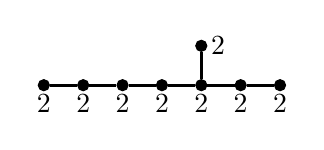
\begin{tikzpicture}
			\tikzset{dynode/.style={circle, draw, fill=black,
						minimum size=4pt, inner sep=0pt}}
			\tikzset{dyline/.style={line width=1pt}}
			\tikzset{dydash/.style={line width=1pt, dashed}}

			\begin{scope}[yshift=-10em, xshift=0]
				\node[dynode] (a1) at (0,0) {};
				\node[dynode] (a2) at (0.5,0) {};
				\node[dynode] (a3) at (1,0) {};
				\node[dynode] (a4) at (1.5,0) {};
				\node[dynode] (a5) at (2,0) {};
				\node[dynode] (a6) at (2.5,0) {};
				\node[dynode] (a7) at (3,0) {};
				\node[dynode] (a8) at (2,0.5) {};

				\draw[dyline] (a1) -- (a2) -- (a3) -- (a4) -- (a5) -- (a6) -- (a7);
				\draw[dyline] (a5) -- (a8);

				\node[below] () at (a1) {$2$};
				\node[below] () at (a2) {$2$};
				\node[below] () at (a3) {$2$};
				\node[below] () at (a4) {$2$};
				\node[below] () at (a5) {$2$};
				\node[below] () at (a6) {$2$};
				\node[below] () at (a7) {$2$};
				\node[right] () at (a8) {$2$};
			\end{scope}
		\end{tikzpicture}
		\quad\implies\quad
		\begin{pmatrix}
			2 & 1 &   &   &   &   &   &   \\
			1 & 2 & 1 &   &   &   &   &   \\
			  & 1 & 2 & 1 &   &   &   &   \\
			  &   & 1 & 2 & 1 &   &   &   \\
			  &   &   & 1 & 2 & 1 & 0 & 1 \\
			  &   &   &   & 1 & 2 & 1 & 0 \\
			  &   &   &   & 0 & 1 & 2 & 0 \\
			  &   &   &   & 1 & 0 & 0 & 2 \\
		\end{pmatrix}
	\]
	where each vertex of the tree is weighed by $2$.
\end{proposition}

It's interesting to note that if $Q$ is a matrix associated to a tree $T$, then $P(Q)$ has a $1$-skeleton homotopy equivalent to $T$. This connection between the $1$-skeleton and plumbing along a tree or graph was first noticed by Hirzebruch. 
It makes sense then why we would care about matrices arising from trees instead of from general graphs which may contain cycles -- cycles break the simple-connectedness of the constructed manifold and are thereby much more complicated to work with.

\pagebreak
\section{Brieskorn Varieties}\label{sec:brieskorn}
\cite{milnor1968hypersurfaces}
\cite{kauffman1987knots}
